\documentclass{article}
\usepackage[paperwidth=18cm,paperheight=10.2cm,margin=0cm]{geometry}
\usepackage{graphicx}
\usepackage{CharisSIL}
\usepackage{tikz}
\pagestyle{empty}
\begin{document}
\noindent
\begin{tikzpicture}[x=1cm,y=1cm]
\path[use as bounding box] (0,0) rectangle (18,10.2);
\node[anchor=north,font=\bfseries\Large,align=center,text width=17cm] at (9,9.85)
{Clean accuracy and corruption sensitivity answer different questions};
\node[anchor=north,align=center,text width=10.8cm,font=\bfseries\large] at (6.0,8.55)
{Exploratory JPEG-95 matched-clean design};
\node[anchor=south west,inner sep=0] at (0.35,2.70)
{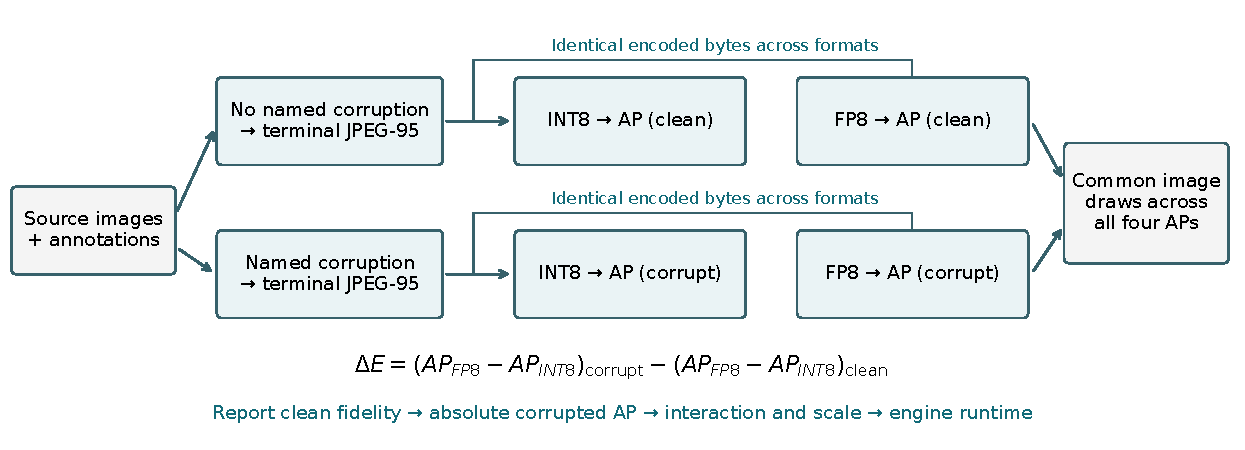
\includegraphics[width=11.25cm]{source/figures/fig_framework.pdf}};
\draw[rounded corners=2mm,line width=0.5pt] (12.05,1.55) rectangle (17.65,8.55);
\node[anchor=north,align=center,text width=5.0cm,font=\bfseries\large] at (14.85,8.25)
{Final VOC/KITTI holdouts};
\node[anchor=north,align=center,text width=5.0cm,font=\footnotesize] at (14.85,7.15)
{Original-source clean\\Six-block means};
\node[anchor=north,align=center,text width=5.0cm] at (14.85,6.25)
{Clean FP8--INT8 gap\\[0.5mm]{\bfseries\Large +1.60 AP}};
\node[anchor=north,align=center,text width=5.0cm] at (14.85,4.95)
{Corrupted FP8--INT8 gap\\[0.5mm]{\bfseries\Large +1.05 AP}\\[-0.5mm]{\scriptsize 95\% paired-image interval: [0.91, 1.16]}};
\node[anchor=north,align=center,text width=5.0cm] at (14.85,3.05)
{Clean-adjusted change\\[0.5mm]{\bfseries\Large -0.55 AP}\\[-0.5mm]{\scriptsize 95\% paired-image interval: [-0.78, -0.29]}};
\node[anchor=south,align=center,text width=17cm,font=\small] at (9,0.35)
{\textbf{Take-home:} FP8 retains higher mean corrupted accuracy in these holdouts,\\
while its clean advantage contracts.\\
Report clean fidelity $\rightarrow$ corrupted AP $\rightarrow$ paired interaction $\rightarrow$ scale/runtime sensitivity.};
\end{tikzpicture}
\end{document}
